\documentclass{mcmthesis}
\usepackage{booktabs}
\usepackage{caption}
\usepackage{graphicx}
\usepackage{subfigure}
\usepackage{threeparttable}
\usepackage{palatino}
\usepackage{lipsum}
\usepackage{longtable}
\usepackage{multirow}
\usepackage[section]{placeins}

\mcmsetup{CTeX = false,   % 使用 CTeX 套装时,设置为 true
        tcn = 75727, problem = A,
        sheet = true, titleinsheet = true, keywordsinsheet = true,
        titlepage = false, abstract = true}
\usepackage{palatino}
\usepackage{lipsum}
\title{Multi-hops HF Radio Wave Propagation}
\author{\small \href{http://www.latexstudio.net/}
  {
\includegraphics[width=7cm]{mcmthesis-logo}}}
\date{\today}
\begin{document}
\begin{abstract}
Shortwave communication are widely used in military, meteorology, commerce and other fields. In order to study multi-hop radio propagation process, we aim to construct models to investigate the reflection and propagation of radio waves on the ocean surface.

Firstly, we build a model for signal reflection off the calm and turbulent ocean, respectively. In model for calm ocean, we can figure out field strength of reflex point after calculating loss. 

Comparing the results of two preceding models, at the same incident angle, the field strength on calm ocean surface is less than the turbulent ocean. At a specific angle, when the signal to noise ratio is less than 10dB, using the field strength formula and the signal to noise ratio, we get the maximum number of hops is 2.

Secondly, in order to precisely calculate the reflection loss on turbulent ocean, we build a Polarization coefficient weight model, In this model, we used Gaussian distribution to simulate the slope distribution of the ocean waves.Based on the slope distribution, we get the weights on the horizontal and vertical polarization coefficient and calculate the reflex loss.

Thirdly, we calculate the field strength and SNR to evaluate the intensity of reflex power. The field strength of mountainous terria is less than smooth ground, and the field strength of turbulent ocean is also less than the calm ocean.

Fourthly, considering the travelling boat will receive both skywave and groundwave, we take both into consideration here. We assume the speed of boat is 30km/h. In one-hop mode, the duration of boat can receive the signal is 59.8h. In two-hop mode, the duration of boat can receive the signal is 53.66h.

Finally, we compare and test the models built in each case, and based on the results of our discussions, submitted a short synopsis of HF radio propagation to IEEE.
\begin{keywords}
Skywave Propagation; Ionosphere; HF; Groundwave 
\end{keywords}
\end{abstract}
\maketitle
\tableofcontents
\newpage

\section{Introduction}
\subsection{Restatement of the Problem}
Shortwave communication with good survivability, simple equipment, good anti-interference, low cost and easy to use, are widely used in military, meteorology, commerce and other departments. Shortwave communications mainly through the ionospheric reflection with the ground for long-distance communications. In this paper, the problem we need to solve is shown as following,
\begin{itemize}
\item Build a model for radio signal propagation on the ocean surface. This part can be divided into two sub-problems. On the one hand, we need calculated 
the strength of a first reflection off a calm and turbulent ocean, respectively. And thereafter compare two results. On the another hand, at calm ocean, the maximum number of hops is also needed to be calculated before its strength falls below a usable signal-to-noise ratio (SNR) threshold of 10 dB. 
\item Compare HF reflections off mountainous or rugged terrain with smooth terrain. Thereafter, compare the preceding answer with this result.
\item Change model to make ship accommodate a shipboard receiver moving on a turbulent ocean. Then, calculate the time that the ship can remain in communication using the same multi-hop path.
\end{itemize}

\subsection{Overview of Our Work}
\begin{itemize}
\item Firstly, we build a model for signal reflection off the calm and turbulent ocean, respectively. Compare the results of two preceding models.
\item Secondly, we build a polarization coefficient weight model. Based on the slope distribution, we get the weights on the horizontal and vertical polarization coefficient and calculate the reflex loss for turbulent ocean.
\item Thirdly, we calculate the field strength and SNR to evaluate the intensity of reflex power. 
\item Fourthly, we take groundwave and skywave propagation into account as considering the communication of travelling boat.
\item Finally, we compare and test the models built in each case, and based on the results of our discussions, submitted a short synopsis of HF radio propagation to IEEE.
\end{itemize}
\subsection{Assumptions}
To simplify our model, we have some assumptions as following, 
\begin{itemize}
\item We \textbf{only consider skywave propagation} here and \textbf{neglect the influence of groundwave propagation}.
\item Assuming the \textbf{basic free space transmission loss, ionospheric absorption loss, reflection loss on the surface of ocean} are the main loss during calculating field strength. Other factors are neglected.
\item Assuming that the reflection of the radio waves in the ionosphere occurs in the E-layer.
\item We neglect the effect of time on ionospheric electron concentration, assuming that \textbf{the electron concentration in the ionosphere E remains constant}.
\end{itemize}
\subsection{Notation}
In order to facilitate the modeling of the model, some variables and symbols are introduced, shown in Table 1.
 \begin{longtable}{c  l c}
 \caption{Variable and Notation} \\
  \toprule
  Abbreviation & Description & Unit\\
  \midrule
  $n_0$ & Refractive index of air\\
   $m$ & Maximum number of hops \\
  $K$ & A constant, is equal to 80.5\\
 $N$ & Electron density of the ionosphere & $m^3$ \\
  $\phi$ & Angle of incidence of radio waves & degree \\
  $D$ & Length of a communication line & $km$\\
  $h'$ & Height between ionosphere and sea   & $km$\\
    $f$ & Reflex frequency from  ionosphere & Hz\\
    $f_{MUF}$ & The highest available frequency & MHz\\
    $\lambda$ & Wave length of radio wave & m\\
    $\theta$ & Incidence angle at 100km height & degree \\
    $f_H$ & Magnetic rotation frequency & MHz\\
    $I_j$& Absorption index \\
    $\chi$ & Reflection of the sun's zenith point &\\ 
    $r$ & Slope distance & km\\
     $\varepsilon_r$ & Complex relative permittivity of ocean\\
     $\sigma$ & Conductivity of the sea surface & $\Omega \bm\cdot m^{-1}$ \\
     $\varphi_1$ & Elevation angle & degree \\
     $E$ &Field strength & $dB(1\mu V/m)$ \\
     $d$ & Single jump distance & km\\
  \bottomrule
 \end{longtable}
 
 \section{Skywave Propagation on the Ocean}
\textit{Radio} is the technology of using radio waves to carry information, such as sound, by systematically modulating properties of electromagnetic energy waves transmitted through space, such as their amplitude, frequency, phase, or pulse width.

\subsection{Model for Calm Ocean}

\subsubsection{Find Maximum Usable Frequency}
 At a certain time, the maximum power transmitted and received by the ionosphere between the transmitting and receiving ends depends on the reflectivity of the ionosphere. When the frequency exceeds this frequency, the radio wave will penetrate the ionosphere but will not return to the ground. The radio frequency at this time is called the basic maximum usable frequency(\textbf{MUF}) $f_{MUF}$. 

Shortwave communications mainly through the ionospheric reflection with ground for long-distance communications, as is depicted in Figure 1. 

When the oblique incidence and vertical incidence of the same height, the frequency of the two waves in line with \textit{the secant theorem}. Now assume that ignoring collisions and magnetic field effects, let $N$ quote electron density of the ionosphere and $f$ quote frequency, the ionosphere has a refractive index $n$$^{[1]}$. 
\begin{equation}
n = \displaystyle\sqrt{1-K\displaystyle\frac{N}{f^2}}
\end{equation}
where $K=80.5$.

Let $\phi$ quote the angle of incidence angle of radio waves, that is, the angle between the direction of incidence of the radio wave and the \textit{Normal}.
The electric wave propagates in the ionosphere and can be derived from \textit{Snell's Law} in the case of plane stratification,
\begin{equation}
n\sin\phi = n_0 \sin\phi_0
\end{equation}
where $\phi_0$ and $n_0$ is the incidence angle and refractive index for radio wave at the bottom of ionosphere, respectively.
\begin{figure}
\begin{minipage}[t]{0.5\linewidth}
\centering
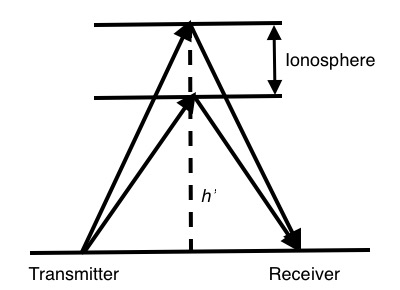
\includegraphics[width=2.4in,height=2.0in]{./figure/layor_reflect.png}
\caption{Ionospheric \protect\\ reflection schematic}
\label{fig:side:a}
\end{minipage}%
\begin{minipage}[t]{0.5\linewidth}
\centering
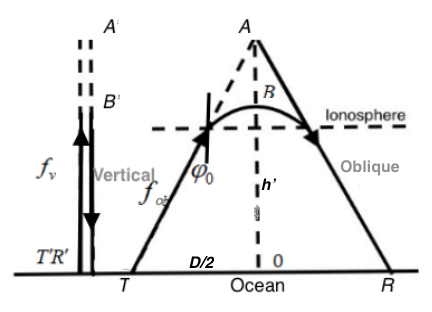
\includegraphics[width=3.in,height=2.4in]{./figure/layor_top.png}
\caption{Equivalent principle of vertical incidence and oblique incidence}
\label{fig:side:b}
\end{minipage}
\end{figure}    

In the atmosphere, let $n_0=1$ and radio wave is reflected at point $B$ (In Figure 2), that is, $\phi=90^\circ$, rearranging Equation (2), we can obtain
\begin{equation} 
n = \sin\phi_0
\end{equation}
 
As for \textbf{vertical incidence}, the hight of reflex point $B'$ is equal to $B$, and $n = 0$ at point $B'$. If let $f_v$ quote the reflex frequency as vertical incidence for the wave, we can obtain from Equation (1), 
\begin{equation}
f_v^2 = KN.
\end{equation}

On the other hand, as for \textbf{oblique incident angle}, at point $B$, let $f_{ob}$ quote the reflex frequency as oblique incident angle for the wave, we can obtain 
\begin{equation}
n = \displaystyle\sqrt{1-K\displaystyle\frac{N}{f_{ob}^2}}
\end{equation}
After combined Equation (3),(4),(5), 
\begin{equation}
f_{ob} = \sec\phi_0 f_v
\end{equation}

According to the geometric relationship in Figure 2,
if let $D$ quote the distance between transmitter(T) and receiver(R), $h'$ quote the height between ionosphere and sea at reflex point, as radio wave oblique incident ionosphere, 
\begin{align}
&f_{ob} = \frac{f_v}{\cos \phi_0} = f_v\displaystyle\sqrt{1+\left( \frac{D}{2h'}\right)^2} \\ 
\Rightarrow ~~ & h'=\displaystyle\frac{f_v D}{2}\sqrt{\frac{1}{f_{ob}^2}-f_v^2} 
\end{align}

If the value of $D$ is certain and the frequency of electric circuit $f = f_{v}$,  we can calculate the relationship between $f$ and $h'$. For example, we set $D=60km$, let $f_{ob}$=10MHz, 12MHz, \ldots , 20MHz, we can obtain the relationship between $h'$ and $f_v$ from Equation (8), as is depicted in Figure 3. 

    \begin{figure}
\begin{minipage}[t]{0.5\linewidth}
\centering
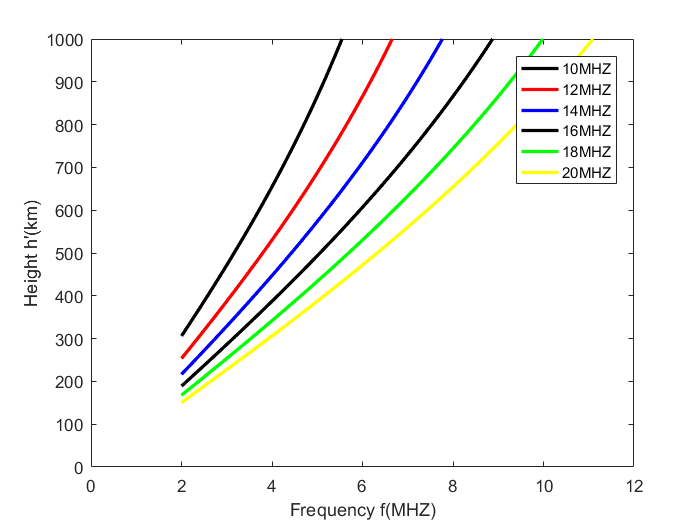
\includegraphics[scale=0.45]{./figure/2.png}
\caption{Communication line  \protect\\ transmission curve as $D$=60km}
\label{fig:side:a}
\end{minipage}%
\begin{minipage}[t]{0.5\linewidth}
\centering
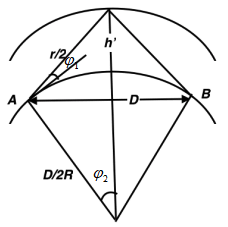
\includegraphics[scale=0.4]{./figure/hh.png}
\caption{Skywave propagation distance}
\label{fig:side:b}
\end{minipage}
\end{figure}   
    
    \subsubsection{Field Strength Calculation}
In the shortwave propagation, the energy loss mainly comes from three aspects,
\begin{itemize}
\item $L_{bf}$ is free space transmission loss;
\item $L_i$ is ionospheric absorption loss;
\item $L_o$ is reflex loss on the surface of ocean or ground. 
\end{itemize}

Other losses (polarization losses and so on) are usually referred to as additional system losses. Since transmit power is 100w (very small), to make the results of our model look more explicit, we only consider three main losses.

\textbf{Free Space Transmission Loss}

When the radio wave propagates in free space, the radio wave moves away from the launch point. The energy radiated by the antenna spreads in more and more large space, making the energy density of radio waves smaller and smaller. The receiver field strength gradually increases with the distance decrease.

The power $P_t$ radiated by the transmitting antenna of the gain $G_t$, after propagating $r$ distance in free space, receives the power at the receiving antenna end of the gain $G_r$ as $P_r$$^{[1]}$. 
\begin{equation}
P_r = \displaystyle\frac{P_tG_t}{4\pi r^2}G_r
\bm\cdot \frac{\lambda^2}{4\pi}
\end{equation}

If we let $L_{bf}$$^{[1]}$ quote basic free space transmission loss, we define it as,
\begin{align}
L_{bf} &= 20\mathrm{lg}(4\pi r)\bm\cdot \frac{4\pi}{\lambda^2}\nonumber\\
&=20\mathrm{lg}(4\pi r)+20\mathrm{lg} f-20\mathrm{lg} c\nonumber\\
&=32.44+20\mathrm{lg}f + 20\mathrm{lg}r
\end{align}
where \begin{itemize}
\item $r$ is slope distance; 
\item $R_0$ is the earth radius and it is equal to 6371km.
\end{itemize}
\begin{equation}
r = 2R_0\displaystyle\sum\limits_{1}^n\frac{\sin(\displaystyle\frac{d}{2R_0})}{\cos\left( \varphi_1+\displaystyle\frac{d}{2R_0} \right)}
\end{equation}
\begin{equation}
\varphi_1 = \arctan(\cot\frac{d}{2R_0}-
\frac{R_0}{R_0+h'}\mathrm{cosec}\frac{d}{2R_0})
\end{equation}
where $d$ is the single hop distance,
\begin{equation}
d = D/n.
\end{equation}
We can figure out the distance $D$ between transmitter and receiver by these formulas,
\begin{equation}
D = \varphi_2\times 111.17,
\end{equation}
\begin{equation}
\cos\varphi_2 = \sin x_1\sin x_2+\cos x_1\cos x_2\cos(y_1-y_2),
\end{equation}
where \begin{itemize}
\item $x_1$ is the latitude of transmitter;
\item $x_2$ is the latitude of receiver;
\item $y_1$ is the longitude of transmitter;
\item $y_2$ is the longitude of the receiver.
\end{itemize}

\textbf{Ionospheric Absorption Loss}

When the shortwave reaches the receiving point through the ionospheric reflection, the energy of the radio wave receives a certain loss due to the penetration and reflection absorption of the absorbing layer, we define it as $L_i$$^{[2]}$.
\begin{equation}
L_i = \frac{677.2\sec \theta}{\left( f+f_H\right)^{1.98}+10.2}
\sum\limits_{j=1}^nI_j ~(dB) 
\end{equation}
where \begin{itemize}
\item $\theta$ quotes incidence angle at 100km height;
\item $f_H$ quotes gyromagnetic frequency;
\item $I_j$ is the absorption index.
\end{itemize}
\begin{equation}
\theta = \arcsin (0.985\cos\varphi_1) 
\end{equation}
\begin{equation}
I_j = (1+0.00037\overline{R}_{12})(\cos0.881\chi)^{1.3}
\end{equation}
In this formula, $\overline{R}_{12}$ quotes the average of sunspot flow over 12 months, $\chi$ quotes reflection of the sun's zenith point. 

The  latitude and longitude of reflect point and local time calculation method can be described as,
\begin{align}
z_k &= 90-\arccos(\cos\lambda_k\sin x_1+
    \sin\lambda_k\cos x_1\cos\phi_3)\\
w_k &=y_1-\arccos \frac{ \cos\lambda_k-\sin z_k\sin x_1 }{\cos z_k\cos x_1} \\
t &= t_0 + (w_k-120)\times 4\mathrm{min}
\end{align}
where
\begin{itemize}
\item $z_k$ is geographic latitude of the $kth$ reflex point;
\item $w_k$ is geographic longitude of the $kth$ reflex point;
\item $\phi_3$ is a azimuth angle from transmitter to receiver;
\item $\lambda_k$ is the center of earth between the $kth$ reflex point and transmitter;
\item $D_k$ is the straight line distance corresponding between transmitter and receiver to $\lambda_k$;
\item $k$ is $kth$ reflex point, among 1$\sim$n;
\item $t$ is the local time at reflex point;
\item $t_0$ is standard time in China.
\end{itemize}
\begin{align}
\cos\phi_3 &= (\sin x_2-\sin x_1\cos\phi_2)/\cos x_1 \sin \phi_2 \\
D_k &= D(sk-1)/2n \\
\lambda_k &= B_k/111.17
\end{align}

\textbf{Reflex Loss}

Reflex loss is only over two hops and after the sea surface reflection mode of transmission there. Assuming that the radiated sky waves are randomly polarized, the radio energy is equally distributed in the horizontal and vertical polarization fields. In symbols, the reflex loss $L_o$$^{[3]}$ can be formatted as 
\begin{equation}
L_o = 10\mathrm{lg}\displaystyle\frac{|R_V|^2 + |R_H|^2}{2}~ (dB) 
\end{equation}
In preceding formula, $R_V$ is the vertical polarization reflection coefficient; $R_H$ is the horizontal polarization reflection coefficient. We can use these two formula to calculate them, respectively.
\begin{align}
R_V &= \displaystyle\frac{\varepsilon_r'\sin \varphi_1-\sqrt{\varepsilon_r'-\cos^2\varphi_1}}{
\varepsilon_r'\sin \varphi_1+\sqrt{\varepsilon_r'-\cos^2\varphi_1}
}\\
R_H &= \frac{\sin \varphi_1-\sqrt{\varepsilon_r'-\cos^2\varphi_1}}{
\sin \varphi_1+\sqrt{\varepsilon_r'-\cos^2\varphi_1}}
\end{align}
where $\varphi_1$ is the elevation angle of radio wave; $\varepsilon_r' = \varepsilon_r - j60\lambda\sigma$, $\sigma$ is the conductivity of the sea surface. We can get the value of $\varepsilon_r$ for different surface in Table 2 (Note that we will use this table again in the second problem). 
\begin{longtable}{l cccc}
\caption{Scope and average of $\varepsilon_r$ and $\sigma$ for different surface} \\
\toprule
 \multirow{2}{*}{Surface} & \multicolumn{2}{c}{Change scope} & \multicolumn{2}{c}{Average} \\
\cmidrule(lr){2-3} \cmidrule(lr){4-5}
     & $\varepsilon_r$  & $\sigma/(\Omega\bm\cdot m)^{-1}$   & $\varepsilon_r$  & $\sigma/(\Omega\bm\cdot m)^{-1}$ \\
\midrule
Seawater  & 80 & $1\sim 4.3$ & 80 & 4    \\
Freshwater  & 80 & $10^{-3}\sim 2.4\times 10^{-2}$ & 80 & $10^-3$ \\
Wet soil & $10\sim 30$ & $3\times 10^{-3}\sim 2.4\times 10^{-2}$ & 10 & $10^{-2}$ \\
Dry soil & $3 \sim 4$ & $1.1\times 10^{-5}\sim 2\times 10^{-2}$ & 4 & $10^{-3}$\\
\bottomrule
\end{longtable}


In physics, field strength means the magnitude of a vector-valued field. We can calculate the field strength $E$$^{[1]}$ of this model, 
\begin{equation}
E = 136.6+P_t+G_t+20\mathrm{log} f-L_{bf}-L_i-L_o. 
\end{equation}
where $f$ is the propagation frequency (MHz); $P_t$ is transmit power.
   \subsubsection{Intensity of the First Reflection of the Calm Ocean}
Due to time and equipment limitations, we choose to use experimental data$^{[4]}$ from other papers. 
In the sea area around Taiwan Island in the South China Sea, 200km from the launch point (20N, 115E) as receiving point. The working frequency is the highest usable frequency, so we can calculate the strongest skywave field strength (use the process in Figure 5). 

In the preceding assumption, we assume the average number of sunspots is a constant. And some basic elements can be calculated. 
Algebraically, it is easy to verify that
\begin{equation}
\overline{R}_{12} = 100, ~\varphi_3 = 41^\circ,~G_t=1
\end{equation}

\begin{figure}[!htbp]
    \centering
    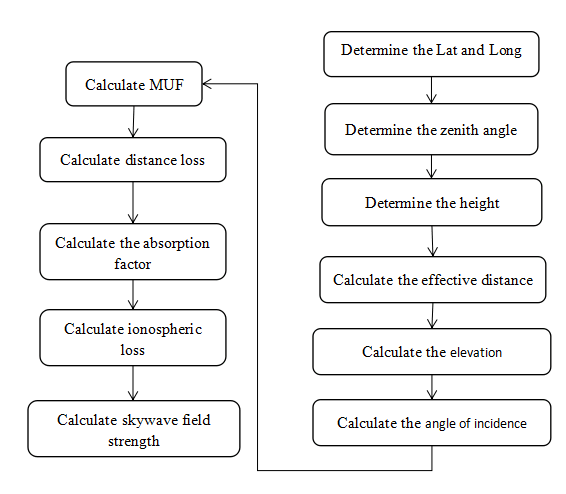
\includegraphics[scale=0.6]{figure/process.png}
    \caption{Field strength calculation flow}
    \label{fig:myphoto55}
    \end{figure}
  
\subsection{Model for Turbulent Ocean}
When we calculate the reflection loss of calm ocean, we assume the radio energy is \textbf{equally} distributed in the horizontal and vertical polarization fields. 
However, this condition can't be applied to turbulent ocean. 
If we figure out \textbf{the weight of horizontal ($w_x$) and vertical polarization ($w_y$)} by slope, respectively, reflection loss $L_o'$ for turbulent ocean can be calculated by this formula,
\begin{equation}
L_o' = 10\mathrm{lg}\displaystyle\frac{w_x\bm\cdot|R_V|^2 + w_y\bm\cdot|R_H|^2}{w_x+w_y} ~(dB).
\end{equation}
\subsubsection{Calculate Reflection Loss}
The Cox-Munk probability density function (PDF) for slopes ($\gamma_x$, $\gamma_y$) of wind-driven ocean waves was obtained about 50 years ago and until now has remained the most complete result. The PDF is widely used in different applications. Herein a method based on the decomposition of an arbitrary PDF in the sum of displaced Gaussian functions is employed. 

We assume that the mean wind vector $w$ is directed along the positive $y$ axis, and the $x$ axis is directed in a crosswind direction. Mathematically, we can get the water surface equation has the form 
\begin{equation}
z = \zeta (x,y),
\end{equation}
the slopes $\gamma_x$ in the $z$ direction and $\gamma_y$ in the $y$ direction are defined by the formulas
\begin{equation}
\gamma_x = \frac{\partial \zeta(x,y)}{\partial x}, \quad
\gamma_y = \frac{\partial\zeta (x,y)}{\partial y}.
\end{equation}

We denote $P(x,y)$ as the joint PDF of principal slopes. It is clear that the probabilities of positive and negative slopes in the crosswind directions are equal because none of them takes preference. Thus, we can obtain
\begin{equation}
P(-\gamma_x, \gamma_y) = P(\gamma_x, \gamma_y).
\end{equation}

In Cox and Munk the truncated Gram-Charlier expansion was used for describing $P(\gamma_x, \gamma_y)$$^{[5]}$:
\begin{equation}
P_{CM}(\gamma_x, \gamma_y) \approx \frac{G_4(\xi. \eta)}{2\pi \sigma_c\sigma_u}\bm\cdot\mathrm{exp}\left( -\frac{\xi^2+\eta^2}{2} \right),
\end{equation}
where 
\begin{equation}
\xi = \frac{\gamma_x}{\sigma_c},\quad \eta = \frac{\gamma_y}{\sigma_u}
\end{equation}
and $G_4(\xi, \eta)$ is some polynomial with respect to $\xi, \eta$:
\begin{align}
G_4(\xi, \eta) =& 1-\frac{1}{2}c_{21}(\xi^2-1)\eta-\frac{1}{6}c_{03}(\eta^3-3\eta) \nonumber
 + \frac{1}{24}c_{40}(\xi^4-6\xi^2+3) \nonumber\\
& + \frac{1}{4}c_{22}(\eta^2-1) \nonumber + \frac{1}{24}c_{04}(\eta^4-6\eta^2+3). 
\end{align}
In accordance with Equation (32), the variable $\gamma$ enters in Equation (33) and (35) only in the form $\xi^2$. All the parameters $\sigma_c, \sigma_u, c_{21}, c_{03}, c_{40}, c_{22}$ and $ c_{04}$ may depend on the wind speed $W$. These parameters were determined in Cox and Munk (1954a,b; 1956) for the range of $W$ between 1 and 15 $m\bm\cdot s^{-1}$ and are presented for a clean surface in Equation (36),
\begin{align}
\sigma_c &=\sqrt{0.003 + 0.00192W \pm 0.0002}, \nonumber\\
\sigma_u &= \sqrt{0.00316W \pm 0.004},\nonumber\\
c_{21} &= 0.01 - 0.0086W\pm 0.03,\nonumber\\
c_{03} &= 0.04 - 0.033W \pm 0.12,\nonumber\\
c_{40} &= 0.40 \pm 0.23,\nonumber\\
c_{22}& = 0.12 \pm 0.06,\nonumber\\
c_{04} &= 0.23 \pm 0.41.
\end{align}

The equation $G_4(\xi, \eta) = 0$ determines the curve in the $\gamma_x-\gamma_y$ plane, which separates the region of positive and negative value of $G$ (In Figure 6).
If we present the region of slopes for $W=14.5m\bm\cdot s^{-1}$, in which the truncated Gram-Charlier approximation (34)-(35) leads to negative probabilities.
\begin{figure}[!htbp]
    \centering
    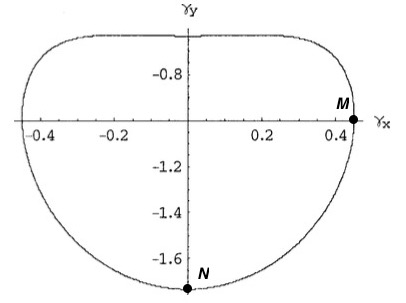
\includegraphics[scale=0.4]{figure/slope.jpeg}
    \centering
    \caption{The domain $G$ in the $\gamma_x-\gamma_y$ plane, where the Gram-Charlier approooximation of the PDF of slopes is negetive for $W = 14.5m\bm\cdot s^{-1}$}
    \label{fig:myphoto1}
    \end{figure}
    
From Figure 6, we can evaluate the weight of horizontal $w_x$ (at M point) and vertical polarization $w_y$ (at N point), respectively. Algebraically, we can obtain
\begin{equation}
w_x \approx 1.8,\quad w_y \approx 0.5
\end{equation}

So we can obtain multi-hop sea-surface reflection loss $L_o'$ for turbulent ocean,
\begin{equation}
L_o' = 10\mathrm{lg}\displaystyle\frac{1.8\bm\cdot|R_V|^2 + 0.5\bm\cdot|R_H|^2}{2.3} ~(dB).
\end{equation}

Now we can calculate the field strength $E'$ on the receiving point  if ocean is turbulent, 
\begin{equation}
E' = 136.6+P_t+G_t+20\mathrm{log} f-L_{bf}-L_i-L_o'. 
\end{equation}
\subsubsection{Intensity of the First Reflection of the Turbulent Ocean}

According to the flowchart process to calculate the results from Figure 5, and combine with Equation (10), (16),  (25), (28), (39), (40), finally we can figure out the value of $L_{bf},L{i},L_o,E,L_o',E'$ by using different incident angle, the result is depicted in Table 3 (the unit of distance is $km$, the unit of loss is $dB$). 

 \begin{longtable}{r  cccccccccc}
 \caption{Intensity of the first reflection of the calm and turbulent ocean} \\
  \toprule
  Incident angle & 0$^\circ$&   15$^\circ$&  30$^\circ$&  45$^\circ$&  60$^\circ$&  75$^\circ$ \\
  \midrule
Propagation distance &   1794.01&    645.86&  304.69&  176.44&  101.54  &46.31\\
Distance loss $(L_{bf})$ &  156.01&  114.05 & 108.49 & 105.54 & 103.82 & 102.90  \\
Ionoshpere loss $(L_{i})$ &10.30 &  5.64 &   3.36  &  2.46  &  2.03   & 1.84   \\

Field strength $(E)$ & 98.41 &  143.24 & 150.94 & 154.75 & 156.89 & 158.01 \\
Field strength $(E')$  &100.39 &    143.43 &    151.02 &    154.79&     156.91 &    158.01   \\
Reflex loss $(L_o)$ & 2.17 &   0.37   & 0.24   & 0.20    &0.20   & 0.19   \\
Reflex loss $(L_{o}')$& 4.15  &  2.57  &  0.32 &   0.24   & 0.21 &   0.20  \\
SNR (calm) & 19.86 &  23.12  & 23.58 &  23.79 &  23.91 &  23.97   \\
SNR (turbulent) &20.03&   23.13  & 23.58 &  23.79 &  23.91 &  23.97 \\
  \bottomrule
 \end{longtable}

\textbf{Comparing turbulent ocean with calm ocean in reflex process: } Table 3 shows the field strength on calm and turbulent ocean, respectively. And the both of field strength will increase as incident angle increases, and their distance loss, ionosphere loss are steady. However, at the same incident angle, the field strength at the receiving point of the \textbf{calm ocean} surface, is \textbf{less than} the \textbf{turbulent ocean} surface. The main reason is that the reflex loss by the turbulent surface ocean is larger than the another one. According to Equation (28),(40), reflex loss is larger, so the field strength at receiving point is smaller.

\subsection{Maximum Number of Hop}
We neglect the extra loss, so our result must have some error. As a consequence, we can figure out field strength and SNR by using different incident angle in the reflex process. \textbf{If its strength falls below a usable signal-to-noise ratio (SNR) threshold of 10dB, we just stop calculate this process and figure out the maximum number of count}, as is depicted in Table 4. 
\newpage
\begin{longtable}{c cccccc}
\caption{Field strength and SNR in reflex process} \\
\toprule
  Incident angle & 0$^\circ$&   15$^\circ$&  30$^\circ$&  45$^\circ$&  60$^\circ$&  75$^\circ$ \\
\midrule 
Field strength of 1th reflex& 98.41 &  143.24 & 150.94 & 154.75 & 156.89 & 158.01  \\
\textbf{SNR of 1th reflex}
& \textbf{19.86} &  \textbf{23.12}  & \textbf{23.58} &  \textbf{23.79} &  \textbf{23.91} & \textbf{23.97}   \\
Field strength of 2th reflex
&13.24&42.89&54.65&60.88&64.37&66.03  \\
\textbf{SNR of 2th reflex}
&\textbf{2.44}&\textbf{11.15} &\textbf{14.23} &\textbf{15.44} &\textbf{16.04} &\textbf{16.34} \\
\bottomrule
\end{longtable}

\begin{figure}[!htbp]
    \centering
    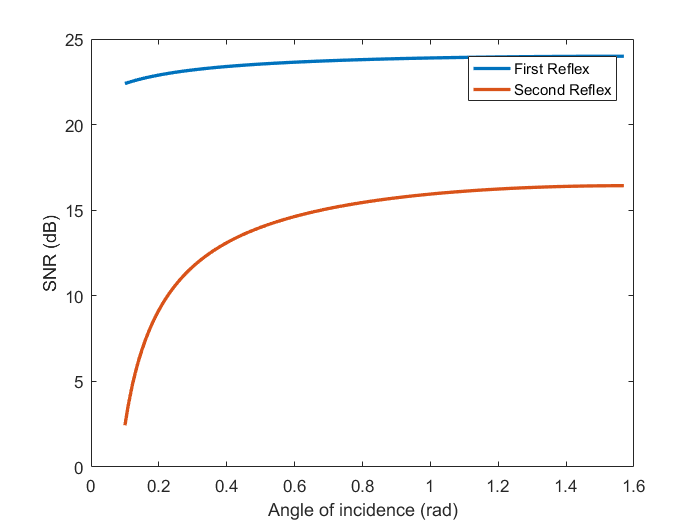
\includegraphics[scale=0.5]{figure/angle_SNR.png}
    \caption{The relationship between the incident angle and SNR}
    \label{fig:myphoto12}
    \end{figure}
Therefore, 
we figure out that the signal can take \textbf{two} hops before its strength falls below a usable signal-to-noise ratio (SNR) threshold of 10dB.
By the way, 
 if the incident angle is larger than \textbf{0.23rad} (13.18$^\circ$), there is a good chance of a second and above jump, as is depicted in Figure 7.
   \subsection{Sensitivity Analysis}
   \subsubsection{ Frequency and SNR}
   We can figure out the relationship between frequency and SNR in different hops, as is depicted in Figure 8.
    We find that in the low range of frequency, the change of frequency will cause a great influence on the SNR, with the value of frequency increasing to 10MHZ, and the SNR will become very steady.
   \begin{figure}
\begin{minipage}[t]{0.5\linewidth}
\centering
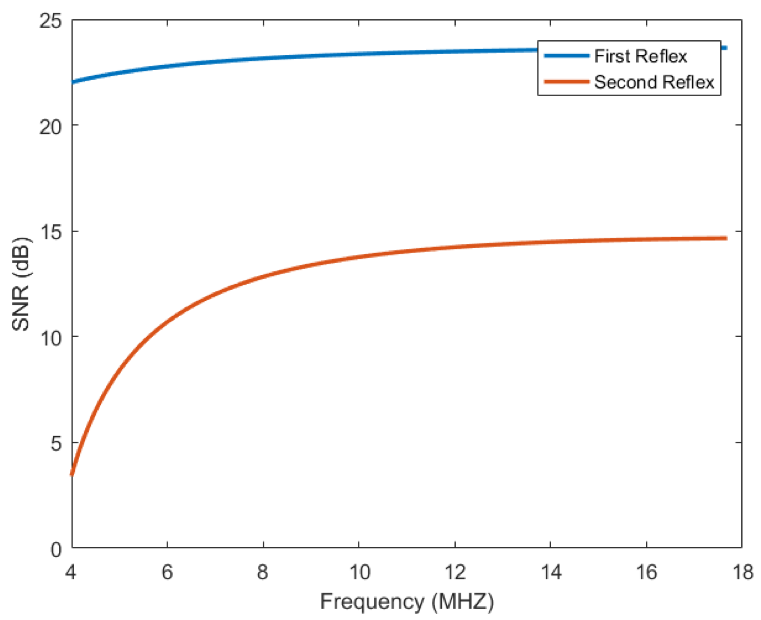
\includegraphics[width=2.8in,height=2in]{figure/sen_1.png}
   \caption{The relationship between\protect\\ the Frequency and SNR on the \protect\\turbulent ocean}
     \label{fig:side:a}
\end{minipage}%
\begin{minipage}[t]{0.5\linewidth}
\centering
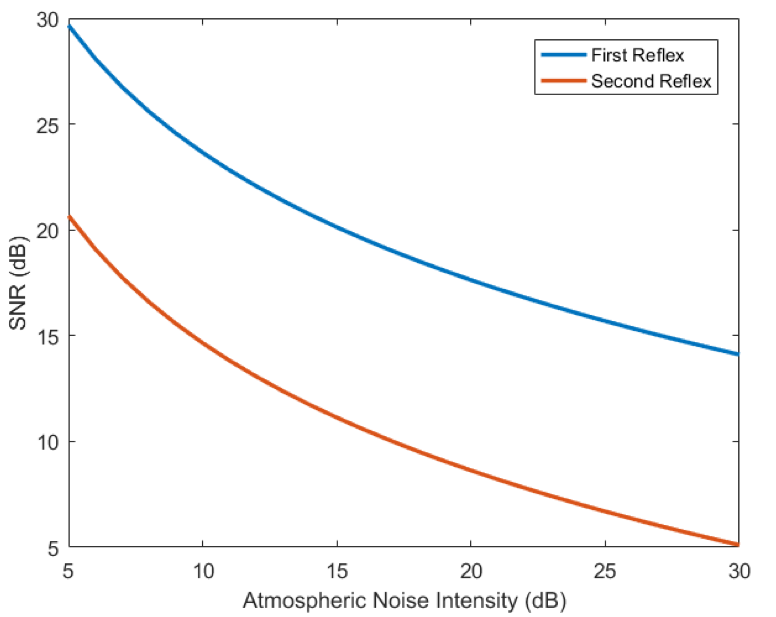
\includegraphics[width=2.8in,height=2in]{sen_2.png}
   \caption{The relationship between the Atmospheric Noise Intensity and SNR on the turbulent ocean}
     \label{fig:side:b}
\end{minipage}
\end{figure}  
   \subsubsection{Atmospheric Noise Intensity and SNR}
SNR is a measure used in science and engineering that compares the level of a desired signal to the level of background noise, which is defined as the ratio of the power $P_{signal}$ of a signal (meaningful information) and the power$P_{noise}$ of background noise (unwanted signal)$^{[8]}$:
\begin{equation*}
SNR = \frac{P_{signal}}{P_{noise}},
\end{equation*}   

In this problem, $P_{signal}=P_t=100w$, so
   we can figure out the relationship between Atmospheric Noise Intensity and SNR, as is depicted in Figure 9. 
We find that with the increasing of the Atmospheric Noise Intensity, the value of SNR will decrease rapidly. So it's obvious that the Atmospheric Noise Intensity take an important role in the SNR calculation. And the determination of Atmospheric Noise Intensity would be better if we search this basing on the real position (Longitude and Latitude).
    
\section{Reflex on the Ground}
\subsection{HF Reflections off Smooth Terrain}
In the preceding Table 2, we show relative permittivity $\varepsilon_r$ and surface conductivity $\sigma$ of the wet soil and dry soil, respectively. We can calculate reflex loss of the ground,
\begin{equation}
L_g = 10\mathrm{lg}\left( 
\frac{|R_v|^2+|R_H|^2}{2}
 \right)
\end{equation}
where $R_V,R_H$ can be calculated by Equation (26),(27). Now we can calculate field strength $E_1$ and SNR of HF reflections off smooth terrain,
\begin{equation}
E_1 = 136.6+P_t+G_t+20\mathrm{log} f-L_{bf}-L_i-L_g. 
\end{equation}
\subsection{HF Reflections off Mountainous Terrain}
When considering the reflex of the mountainous or rugged terrain, we mainly build the Single Knife-edge Obstacle and Multiple Knife-edge Obstacle for it. In this model, we assume that there is a isolated mountain between the transmitter and receiver. And the height of the mountain is set to 2000m, and the width can be neglected. 

\textbf{Single knife-edge Obstacle Propagation Model}. We can see single knife-edge obstacle propagation more clearly in Figure 11.
  It is obvious that when the skywave reach the mountainous area, the reflex will occur on the back-side of the mountain.  If the skywave from ionosphere reach the middle and bottom part of the mountain, radio wave willl occur diffraction phenomenon. 
\begin{figure}[!htbp]
    \centering
    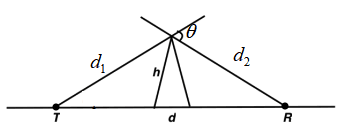
\includegraphics[scale=0.55]{figure/popopo.png}
    \caption{Single knife-edge obstacle propagation}
    \label{fig:myphoto12}
    \end{figure}
    
If let $\nu$ quote twice the height of the obstacle $h$ and the Fresnel radius $F_1$ ratio, mathematically, we can obtain
\begin{align}
\nu = \frac{\sqrt{2}h}{F_1}, \quad
F_1 = \displaystyle\sqrt{\frac{\lambda d_1d_2}{d}} 
\end{align}
Rearranging the Equation (42), we can obtain
\begin{equation}
\nu = \displaystyle\sqrt{\frac{2h^2d}{\lambda d_1d_2}}. 
\end{equation}

The diffraction between the obstacles TR can be expressed as $J(\nu)(dB)$$^{[6]}$ can represented as
\begin{equation}
J(\nu) = 
\begin{cases}
5.7+9\nu + \nu^2 -1.4\nu^3 & -1.8<\nu<1.5 \\\\
12.9+20\mathrm{lg}(\nu) & \nu\geqslant 1.5
\end{cases}
\end{equation}
Now we can calculate field strength $E_2$ and SNR of HF reflections off smooth terrain,
\begin{equation}
E_2 = 136.6+P_t+G_t+20\mathrm{log} f-L_{bf}-L_i-J.
\end{equation}

 \textbf{Multiple Knife-edge Obstacle}. In front of us only considered the case of a mountain, here we have to discuss the situation of multiple hills. To figure out the ridges on the topography that may cause diffraction loss, we mark the mountains $A_1,A_2,\ldots,A_n$.
Let the diffraction loss of each ridge be $J_{Ai}$, and add the individual ridge losses to total loss $J_A$. 
\begin{equation}
J_A = \sum\limits_{i=1}^nJ_{Ai} 
\end{equation}
Rearranging Equation (44), we can obtain
\begin{align}
J_{Ai}  = 
\begin{cases}
5.7+9\nu_i+\nu^2-1.4\nu_i^3 & -1.8<\nu<1.5\\
\\
12.9 + 20\mathrm{lg}(\nu_i) & \nu\geqslant 1.5
\end{cases}
\end{align}
In this formula, if let $H_i$ is the height of mountain $A_i$, we can obtain
\begin{equation}
\nu_i = \frac{\sqrt{2}h_i}{F_1} = \frac{\sqrt{2}(H_i-H_{i-1})}{F_1}
\end{equation}

\subsection{Analysis the Results}
From Equation (40), (41), (47), (45), we can obtain the loss of smooth ground $L_g$, the field strength of smooth ground $E_1$, the loss of mountainous terrain $J$,  the field strength of mountainous terrain $E_2$. We set these result to Table 5.

 From the results Table 5, the loss of mountainous or rugged terrain is much larger than the turbulent ocean. We think the main reason of this situation is the height of mountains is much taller than the ocean wave. So when the skywave reach the mountainous area, the diffraction loss take the dominant role. And the diffraction loss $J$ is usually larger than the reflex loss $L_g$. 
 
\begin{longtable}{r cccccc}
\caption{Field strength and SNR of HF reflections off mountainous and smooth terrain}\\
\toprule
  Incident angle & 0$^\circ$&   15$^\circ$&  30$^\circ$&  45$^\circ$&  60$^\circ$&  75$^\circ$ \\
\midrule 
Reflex loss $(L_g)$& 2.24 & 6.27 & 8.27 & 9.00 & 9.19 & 9.22 \\
Diffraction loss $(J)$ & 36.62 & 36.62 & 36.62 & 36.62 & 36.62 & 36.62 \\

Field strength $(E_1)$& 133.14 & 152.60 & 160.56 & 164.43 & 166.37 & 167.23 \\
Field strength $(E_2)$& 94.27 & 109.71 & 115.67 & 118.81 & 120.56 & 121.39 \\
SNR (Smooth ground)& 22.49 & 23.67 & 24.11 & 24.32 & 24.42 & 24.47 \\

SNR (Mountains) & 19.49 & 20.80 & 21.26 & 21.50 & 21.62 & 21.68 \\
\bottomrule
\end{longtable}

  For ocean waves we can approximately use Gaussian Distribution to simulate it's slope, as the shape of ocean waves is influenced by the wind speed and direction, and which also influence the Complex Relative Permittivity of the ocean uneven distribution. As for the mountains, which are natural formation and it's hard to predict the slope and Complex Relative Permittivity. So we just use Single-Knife Obstacle model to predict the loss of diffraction.
\subsection{Sensitivity Analysis}

\subsubsection{Frequency and SNR}
We can see the relationship between the Frequency and SNR on the mountainous area, as is depicted in Figure 11. It's obvious that the selection of $f$ will cause huge influence on our result, with the increasing of frequency, the SNR will decrease rapidly.  
    \begin{figure}[!htbp]
    \centering
    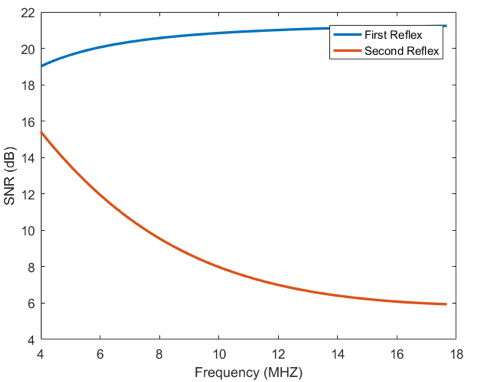
\includegraphics[scale=0.9]{figure/sen_3.png}
    \caption{The relationship between the Frequency and SNR on the mountainous area}
    \label{fig:myphoto12}
    \end{figure} 
    
\subsubsection{Height and SNR}
On the mountainous area, we can see the relationship between the height of the mountains and SNR, as is depicted in Figure 12.
 \begin{figure}[!htbp]
    \centering
    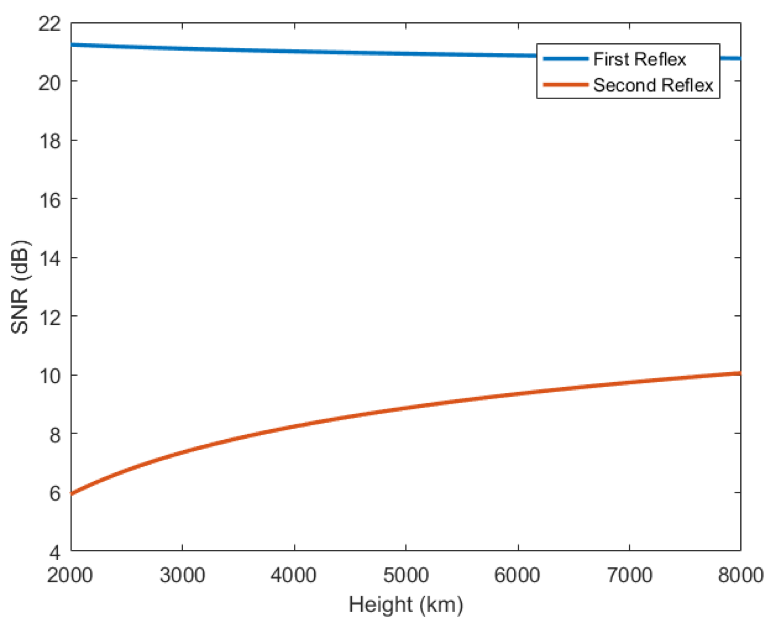
\includegraphics[scale=0.6]{figure/sen_4.png}
    \caption{The relationship between the height of the mountains and SNR on the mountainous area}
    \label{fig:myphoto12}
    \end{figure} 

According to the Figure 12, we find that, the first SNR reflex is relatively stable, but the second reflex SNR will be obviously effected as the hight changes. That is, high intensity shortwave is stable in the mountainous area, but the weak shortwave is exactly the opposite. 

\section{HF Propagation of the Moving Ship on the Ocean }
In the above section, we calculate the largest incident angle is 0.23rad (13.18$^\circ$). If the incident angle is less than 0.23rad, the shortwave will only jump one time. From the previous result, the furthest distance of two-hop mod is 1609.88 and the furthest distance of one-hop is 1794.01. So in the close range of ocean, the boat will receive both the skywave and groundwave, when the boat's travel distance is more than 200km, the skywave take the dominant role. So we will modify our model to adapt the shortwave short-range transmission, and we take the groundwave into our consideration. 
\subsection{Groundwave Propagation}
When the sea surface wave propagation distance within 50km, we can obtain empirical formula$^{[7]}$ as following
\begin{align}
E_n = &116+10\mathrm{lg}P_t-20\mathrm{lg}D-\frac{10}{3}\mathrm{lg}\left( \frac{300}{f} \right)  -10D\left( \frac{300}{f} \right)^{-\frac{3}{2}} ~(dB).
\end{align}
When the sea surface wave propagation distance is within 50$\sim$200km, 
\begin{equation}
E_n = 95+10\mathrm{lg}P_t-10\mathrm{lg}D-\frac{10}{3}\mathrm{lg}\left(\frac{300}{f} \right)-10D\left( \frac{300}{f}\right)^{-\frac{3}{2}}~(dB)
\end{equation}

So in the close distance of ocean, the total field strength is the superposition of the field strength of skywave and groundwave.
\subsection{Calculate Time of Propagation}
 If let $d_f$ quote the furthest distance in different mode, and $\upsilon$ quote the speed of boat, we can calculate the duration $t$ of boat by this formula,
 \begin{equation}
	t = \frac{d_f}{\upsilon }
 \end{equation}
 
\textbf{One-hop mode}. The furthest distance of one-hop mode is 1794.01km, we assume the speed of boat is 30km/h($\upsilon = 30km/h$). So we can obtain the duration that boat can receive the signals is 59.8 hours by Equation (51).

\textbf{Two-hop mode}. The furthest distance of two-hop node is 1609.88km, So we can obtain the duration that boat can receive the signal is 53.66 hours by Equation (51).

\section{Strengths and Weakness}
\subsection{Strengths}
\begin{itemize}
\item \textbf{Easy to calculate}.  Our model doesn't involves many integral or differential calculation.
\item \textbf{Reliable}. We select South China Sea as an instance to calculate all the results and the results conform to the recommended values of the wave propagation mode.
\item \textbf{Technical supporting}.  We use many theory and methods to support our work. And each one of them is used reasonably and properly.
\item \textbf{Good stability}. With the changing of the parameters, the result are very stable, no abnormal value appears.
\end{itemize}
\subsection{Weakness}

\begin{itemize}
\item \textbf{Simple}. We don't take into account many electromagnetic properties of turbulent ocean.
\item \textbf{Simplifying assumption}.  To simplify the model, we make a few assumptions which may affect the results of our model.
\item \textbf{Lack of data}. We don't collect enough data to validate our model, Only according to a recommended range of values to consider the correctness.
\end{itemize}

 \newpage
 \section{Skywave Propagation Model Against the Ocean and Terrain}
 In radio communication, skywave refers to the propagation of radio waves. Since it is not limited by the curvature of the Earth, the skywave propagation is Suitable for long distance communication especially on the ocean environment.
 
From our research, the propagation loss of skywave is mainly affected by the three parts including the free space transmission loss, the ionospheric loss and the reflex loss. We mainly research the reflex loss on the surface of ocean, mountainous area and rugged terrain.

In order to precisely calculate the reflection loss on turbulent ocean, we build a Polarization Coefficient Weight Model.

In this model, we used Gaussian Distribution to simulate the shape of ocean wave based on the wind speed and direction. According to the distribution we assume, we can further get the slope distribution of ocean wave.

 Therefore, we determine the weight of the Horizontal Polarization Component and Vertical Polarization Component. Then we weight the polarization in both directions and using the reflection formula to calculate the reflection loss.
 
Secondly, we calculate the hops that the shortwave can jump. After determining the MUF, to figure out the number of maximum hops, we select the different incident angle to calculate the SNR of the wave. That is, we must continue to calculate SNR of radio wave after reflexed by the surface of ocean. We stop this process until its strength falls below a usable signal-to-noise ratio (SNR) threshold of 10dB.

Thirdly, we are required to make a comparison between the HF reflections off mountainous or rugged terrain versus smooth terrain. So we decide to build a single-knife obstacle model to simulate the skywave propagation and calculate the propagation loss.

In this model, we find that the mountain is a natural formation, and it's hard to using a distribution to describe the distribution of slope. So it is impossible for us to take it into our Polarization Coefficient Weight Model, so we need to build a new model to solve this problem.

In reality, the mountainous area environment is very complex, and it is hard to precisely calculate the propagation loss against it. So we make a strong assumption about the propagation on the mountainous area. We assume most part of the skywave will reach the lower part of the mountains, and transfer to diffract, fewer part of the skywave will reflex on the slope of mountain on the top part. But this part of loss is much smaller than the diffraction loss, and it can be ignored.

Through our research, due to the characteristics of shortwave, when the skywave reach the middle and bottom part of the mountains, the shortwave will start to diffract through the mountains, so we build a single-knife obstacle model to simulate it.

Based on our model, we find that the loss on the mountainous area is much larger than the turbulent ocean, we analyze that the height of mountains is far greater than the ocean waves, and most shortwaves will transfer to diffract and the diffract loss is larger than the reflection loss.

Finally, we begin to consider how does we change our model to accommodate a shipboard receiver moving on the turbulent ocean. Through our analysis, we find that in the offshore range, the ship will mainly receive the strong signals from the groundwave, and the skywave intensity is weak. With the ship leaving the coast, the intensity of skywave will increase and apparently on the 200km department, the shortwave intensity will be too small for shipboard receiver to perceive.

 So we take existing groundwave propagation into our model, and calculate the Superposition intensity,
 In the last part of our work, we calculate the duration of the communication between the wave sender and shipboard receiver when the ship across through the ocean. And we take the South China Sea as an instance to calculate the time in reality.
\newpage
\begin{thebibliography}{99}
\bibitem{1}Xiong Hao. Radio wave propagation [M]. Electronics Industry Press, 2000.627-654
\bibitem{2}Xu Yan. Research and Simulation of Shortwave Sky Wave Channel Characteristics [D]. Harbin Institute of Technology, 2005. 22-22
\bibitem{3}Zhuang Ganbo, Sun Fangang.Analysis on the Influence of Different Ground Forms on HF Communication [J] .New Communications, 2014.1-1
\bibitem{4}Zhang Chaozhu. Research on the technology of maritime short-range short-wave communication system [D]. Harbin Engineering University, 2002.13-16
\bibitem{5}Tatarskii, Valerian I. "Multi-Gaussian representation of the Cox–Munk distribution for slopes of wind-driven waves." Journal of Atmospheric and Oceanic Technology 20.11 (2003): 1697-1705.
\bibitem{6}Liu Liqiang, Song Zhiqun, Chen Dayong.Engineering Approximate Model of Single Knife-edge Diffraction Loss in Mountainous Communication [J] .Proceedings of the CSEE, 2015,41 (1): 24-27.
\bibitem{7}QU Gui-Cheng, WANG Rui.Realiability of Short-Wave Communication over the Sea Under Atmospheric Noise [J]. Ship Electronic Engineering, 2009, 29 (1): 92-95.
\bibitem{8}\url{https://en.wikipedia.org/wiki/Signal-to-noise_ratio}
\end{thebibliography}
\newpage
\begin{appendices}
\section{Source Code of Model Solution }
Solution for SNR in different situations.
\textbf{\textcolor[rgb]{0.98,0.00,0.00}{Input matlab source:}}
\lstinputlisting[language=Matlab]{./code/solution.m}
\end{appendices}
\end{document}
